\documentclass[a4j,11pt]{jarticle}
\usepackage{url}
\usepackage[dvipdfmx]{graphicx}
\usepackage[dvipdfmx]{color}
\usepackage[ipaex]{pxchfon}
\usepackage{listings}
\usepackage{plistings}
\usepackage{color}
\usepackage{amsmath, amssymb}
\usepackage{type1cm}


\definecolor{codegreen}{rgb}{0,0.6,0}
\definecolor{codegray}{rgb}{0.5,0.5,0.5}
\definecolor{codepurple}{rgb}{0.58,0,0.82}
\definecolor{backcolour}{rgb}{0.95,0.95,0.92}
 
\lstdefinestyle{mystyle}{
	language={c},
    backgroundcolor=\color{backcolour},   
    commentstyle=\color{codegreen},
    keywordstyle=\color{magenta},
    numberstyle=\tiny\color{codegray},
    stringstyle=\color{codepurple},
    basicstyle=\footnotesize,
    breakatwhitespace=false,         
    breaklines=true,                 
    captionpos=b,                    
    keepspaces=true,                 
    numbers=left,                    
    numbersep=5pt,                  
    showspaces=false,                
    showstringspaces=false,
    showtabs=false,                  
    tabsize=2
}
 
\lstset{style=mystyle}



\setlength{\textwidth}{1.1\textwidth}
\setlength{\oddsidemargin}{-3pt}
\setlength{\evensidemargin}{\oddsidemargin}
\setlength{\topmargin}{10mm}
\setlength{\headheight}{0mm}
\setlength{\headsep}{0mm}

\newcommand{\argmax}{\mathop{\rm argmax}\limits}
\newcommand{\argmin}{\mathop{\rm argmin}\limits}

\begin{document}

\begin{center}
%\noindent
 \vspace{10mm}

{\bf {\huge 先端機械学習 前半課題}}
%\end{center}

\vspace{80mm}

提出日:2021年 7月28日

\vspace{10mm}

情報工学系

\vspace{10mm}

学籍番号:18B14822

\vspace{10mm}


\vspace{20mm}

{\bf {\LARGE 氏名:宮崎 直哉}}
\end{center}





\newpage




\section{問題1}

\subsection*{パラメータbの値:}

\begin{equation*}
    b = (0, -1000, -1000, -2000, -2000, -3000)
\end{equation*}

\subsection*{パラメータbを求める方法:}
本問題では$w_i = 1000 (i = 1,2,3,4,5,6)$である。この時、シグモイド関数は下図のようになる。この時、このシグモイド関数はステップ関数と考えることができる。

\begin{figure}[hbtp]
    \centering
    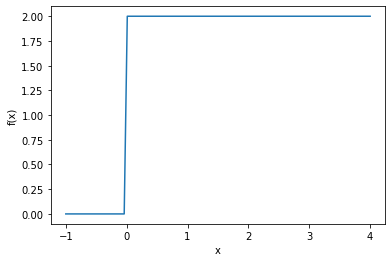
\includegraphics[width=10cm]{p1-3.png}
\end{figure}

この時、$g_i = v_i\sigma(1000x + b_i)$という式の意味を考えてみる。
すると、シグモイド関数はxから[0,1]区間への写像であるので、$v_i$はステップ関数の高さを表すことがわかる。また、
\begin{eqnarray*}
    g_i &=& v_i\sigma(1000x + b_i)\\
    &=& v_i\sigma\left( 1000(x + \frac{b_i}{1000}) \right))
\end{eqnarray*}
と変形すると、$x = -\frac{b_i}{1000}$がステップ関数の変換点となっていることがわかる。例えば、
\begin{equation*}
    f(x) = 
    \left\{
        \begin{array}{ll}
            0 & (x < 3) \\
            5 & (3 \leq x)
        \end{array}
    \right.
\end{equation*}
となるようなステップ関数をシグモイド関数で近似することを考えると、変換点が$x = -\frac{b_i}{1000} = 3$で高さ$v_i=5で$あるので、

\begin{equation*}
    g = 5\sigma(1000x - 3000)
\end{equation*}

とすれば、下図のようにステップ関数をシグモイド関数で近似したグラフを意図して得られる。
\begin{figure}[hbtp]
    \centering
    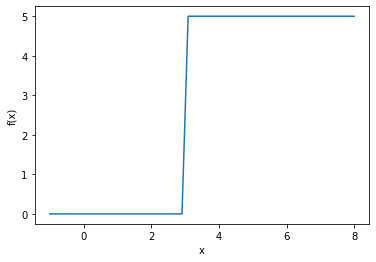
\includegraphics[width=10cm]{p1-4.png}
\end{figure}

\newpage

この性質を利用して本問題を考えてみる。$f(x)$は以下のグラフのようである。
\begin{figure}[hbtp]
    \centering
    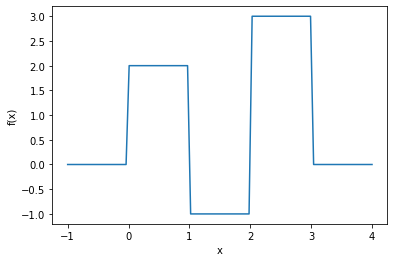
\includegraphics[width=10cm]{p1-2.png}
\end{figure}

式$g(x)$はシグモイド関数の和で表現されているので、上記の性質を合成した関数gを作成することができる。
ここで考えることは、ステップ関数の変換点と高さである。変換点として考えるべきなのは$x = 0,1,2,3$である。高さについては、$x=0:+2$、$x=1:-3$、$x=2:+4$、$x=3:-3$となっている。
高さについては、パラメータvの値を見ていくと、$x=0$において高さ$v_0 = 2$,$x=1$において高さ$v_1 = -2,v_2 = -1$,$x=2$において高さ$v_2 = 1,v_3 = 3$,$x=3$において高さ$v_6 = -3$のステップ関数をそれぞれ適用することで、$||f(x) - g(x)|| < \epsilon$となるようなパラメータbを決定することができる。

\newpage
\section{問題2}

\subsection*{(1)}

\subsection*{(2)}

\newpage
\section{問題3}
RW
WS353


\newpage
\section{問題4}
RNNの代わりにAttentionを用いている

\newpage
\section{問題5}

\end{document}